%%% lorem.tex --- 
%% 
%% Filename: lorem.tex
%% Description: 
%% Author: Ola Leifler
%% Maintainer: 
%% Created: Wed Nov 10 09:59:23 2010 (CET)
%% Version: $Id$
%% Version: 
%% Last-Updated: Wed Nov 10 09:59:47 2010 (CET)
%%           By: Ola Leifler
%%     Update #: 2
%% URL: 
%% Keywords: 
%% Compatibility: 
%% 
%%%%%%%%%%%%%%%%%%%%%%%%%%%%%%%%%%%%%%%%%%%%%%%%%%%%%%%%%%%%%%%%%%%%%%
%% 
%%% Commentary: 
%% 
%% 
%% 
%%%%%%%%%%%%%%%%%%%%%%%%%%%%%%%%%%%%%%%%%%%%%%%%%%%%%%%%%%%%%%%%%%%%%%
%% 
%%% Change log:
%% 
%% 
%% RCS $Log$
%%%%%%%%%%%%%%%%%%%%%%%%%%%%%%%%%%%%%%%%%%%%%%%%%%%%%%%%%%%%%%%%%%%%%%
%% 
%%% Code:


\chapter{Method} \label{cha:method}
  Now that the theoretical groundwork has been laid out, we describe in \cref{sec:implementation} how the solution was implemented into Configura's graphics pipeline and then show how to evaluate it in \cref{sec:evaluation}.
  
\iffalse
 In more detail, the implementation description shows how the different algorithms are implemented in practice and how these fit into Configura's pipeline. Moreover, we also show how the appearance evaluator has been implemented and integrated into the system. In the evaluation part of the method, we describe how to measure the computation time, memory usage, polygon count and appearance preservation of a algorithm given a certain mesh and parameters.
\fi

%%%%%%%%%%%%%%%%%%%%%%%%%%%%%%%%%%%%%%%%%%%%%%%%%%%%%%%%%%%%%%%%%%%%%%
%%
%%% Implementation
%%
%%%%%%%%%%%%%%%%%%%%%%%%%%%%%%%%%%%%%%%%%%%%%%%%%%%%%%%%%%%%%%%%%%%%%%
\section{Implementation} \label{sec:implementation}
In this section an explanation of how the mesh simplification scheme was implemented is given. Some problems that were encountered during the implementation is also presented as well as how they were solved.

\subsection{Handling seams}
To be able to apply a texture to a mesh a mesh parameterization is needed that maps vertices to texture coordinates. If the mesh is not homeomorphic to a disk it is split into parts which will introduce seams. Vertices along these seams is duplicated which enable us to have multiple texture coordinates. However, this is a problem during simplification and will likely make the mesh tear in the seams as seen in \cref{fig:mesh_tear}. Welding duplicate vertices removes the seams and our tearing problem goes away. This, however, does not work good for textured meshes since we can no longer have discontinuities which results in the seam shown in \cref{fig:mesh_discontinuity}. Vertices that share the same attributes are safe to remove though.

\begin{figure}[ht]
  \centering
  \begin{subfigure}[b]{.45\textwidth} 
    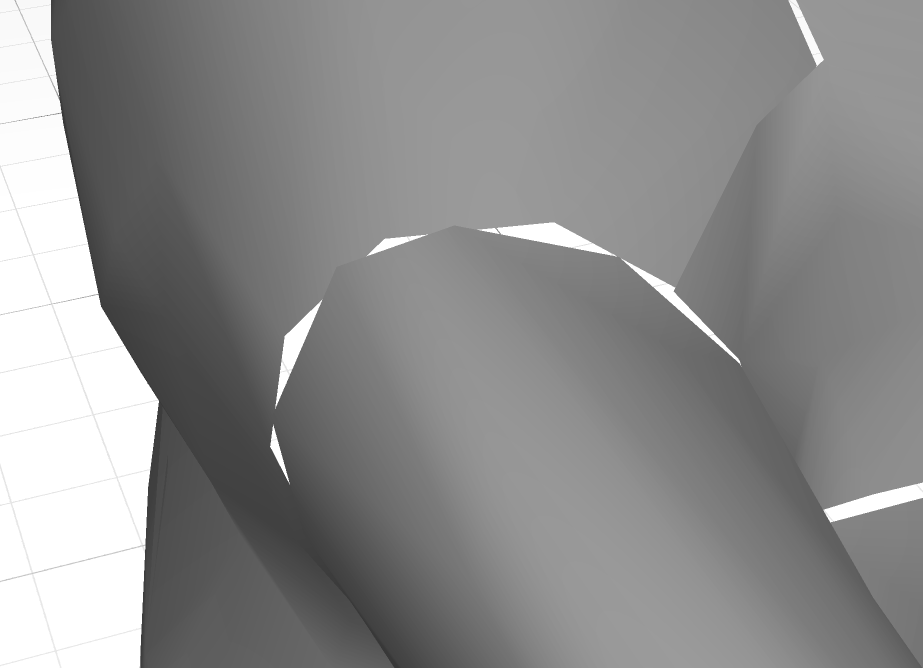
\includegraphics[width=\textwidth]{mesh_tear.png}
    \caption{Mesh tear in seam}
    \label{fig:mesh_tear}
  \end{subfigure}
  ~
  \begin{subfigure}[b]{.45\textwidth}
    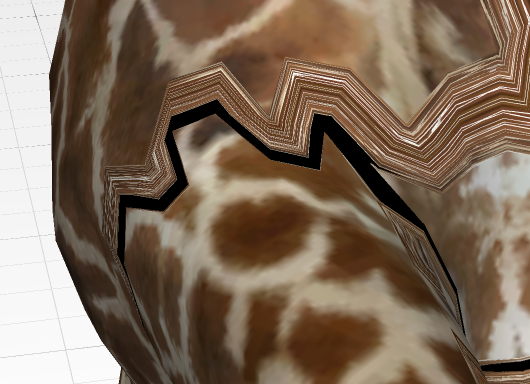
\includegraphics[width=\textwidth]{mesh_remove_duplicates.png}
    \caption{Discontinuity destroyed}
    \label{fig:mesh_discontinuity}
  \end{subfigure}
  \caption{Problems in the seams of a mesh}
  \label{fig:mesh_seam_problems}
\end{figure}

The mesh representation by Hoppe \cite{hoppe1998efficient} allows vertices to have multiple attributes associated with it. As explained in \cref{sec:vertex_with_multi_attributes} the corners of a face defines the attribute value that should be used for that face.

\iffalse
\begin{figure}[ht]
    \centering
    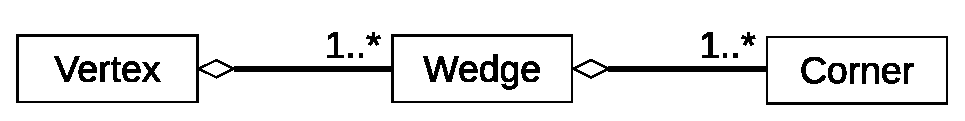
\includegraphics[width=.5\textwidth]{figures/vertex_wedge_corner.eps}
    \caption{Multi-attribute vertex}
    \label{fig:vertex_wedge_corner}
\end{figure}
\fi

\lstset{
  language=C++,
  classoffset=0,
  morekeywords={in,from,to},
  keywordstyle=\bfseries\color{blue},
  commentstyle=\itshape\color{darkgreen},
  morecomment=[l][\bfseries\color{cyan4}]{\#},
  classoffset=1,
  morekeywords={hash,floor,rotateRight,eq,abs,removeDuplicates,quadric,compute_face_quadric,random},
  keywordstyle=\bfseries\color{darkblue},
  classoffset=2,
  emph={int,float,vec2,vec3,bool,double,vector,void,Face,Quadric,point},
  emphstyle={\bfseries\color{darkred}},
  classoffset=3,
  emph={V,U},
  emphstyle={\bfseries\color{black}},
  classoffset=0,
  captionpos=b}

\begin{subs}
\subsubsection{Finding duplicate vertices}
A fast method to find vertices that occupy the same space in 3D is to use a hash map. It is an associative container that is organized into buckets that contains the elements. Search, insert, and removal of elements have on average constant time complexity but in the worst case linear. If a key maps to the same bucket as another key it will be put in a collision chain in the same bucket. The time complexity will in that case be linear on the number of elements in that bucket.

To get fast search and insert a hash function with few collisions is important. The hash function that is used at Configura can be seen in \cref{lst:hash3D}. This hash of a 3-dimensional vector is a combination of the x, y, z coordinates. The hashes of x and y is also rotated i.e. bits are circular shifted, to get fewer collisions. 

\begin{minipage}{\textwidth}
\begin{lstlisting}[caption={Hashing 3D point}, label={lst:hash3D}]
  bool eq(float a, float b) {
    return abs(a - b) < precision;
  }
  
  int hash(float z) {
    if (eq(z, 0.0)) return 0;
    float r = floor(z/precision);
    int* p = (int*)&r;
    return rotateRight(p[0], 4);
  }
  
  int hash(vec3 p) {
    return (rotateRight(hash(p[0]), 8) +
            rotateRight(hash(p[1]), 4) +
            hash(p[2]));
  }
\end{lstlisting}
\end{minipage}

Extracting all \emph{unique} vertices in a mesh can be done with the aformentioned hash map. This is done by iterating through all the vertices and inserting them into the hash map. If the map already contains a vertex we have found a duplicate and it will not be inserted. After the iterations the map will only contain unique vertices and the next step is to update the triangles to map to the new vertices. This is an easy task since when the vertices are inserted into the hash map they will be associated with an index. Therefore, we only have to iterate through the triangle indices and update them with the new indices. (See \cref{lst:remove_duplicates}).

\begin{minipage}{\textwidth}
  \begin{lstlisting}[caption={Removing duplicates}, label={lst:remove_duplicates}]
    void removeDuplicates(vector<vec3>& vertices,
                          vector<int>& triangles) {
      unordered_map<vec3, int> indices;
      vector<vec3> newVertices;
      
      for (vec3 v : vertices) {
        if (!indices.count(v)) {
          indices.emplace(v, newVertices.size());
          newVertices.push_back(v);
        }
      }

      vertices = newVertices;

      // Remap triangles to the new vertices
      for (int i=0; i<triangles.size(); i++) {
        int index = triangles[i]
        vec3 z = vertices[index];
        int newIndex = indices[z];
        triangles[i] = newIndex;
      }
    }
\end{lstlisting}
\end{minipage}

\iffalse
% Too long!? Move to appendix?
\begin{minipage}{\textwidth}
  \begin{lstlisting}[caption={Removing duplicates}, label={lst:remove_duplicates}]
    void removeDuplicates(vector<vec3>& vertices,
                          vector<vec2>& texCoords,
                          vector<int>& triangles) {
      unordered_map<vec3, vector<int>> indices;
      unordered_map<int, int> old_to_new;
      
      vector<vec3> newVertices;
      vector<vec2> newTexCoords;
      
      for (int i=0; i<vertices.size(); i++) {
        vec3 v = vertices[i];
        vec2 t = texCoords[i];
        
        if (!indices.count(v)) {
          vector<int> vec{newVertices.size()};
          indices.emplace(v, vec);
          oldToNew.emplace(i, newVertices.size());
          
          newVertices.push_back(v);
          newTexCoords.push_back(t);
          
        } else {
          vector<int> vec = indices[i];
          
          if (uniqueTexCoord(i, vec)) {
            indices[v].push_back(newVertices.size());
            oldToNew.emplace(i, newVertices.size());
            
            newVertices.push_back(v);
            newTexCoords.push_back(t);
          }
        }
      }

      vertices = newVertices;
      texCoords = newTexCoords;

      // Remap triangles to the new vertices
      for (int i=0; i<triangles.size(); i++) {
        int index = triangles[i];
        triangles[i] = oldToNew[index];
      }
    }
\end{lstlisting}
\end{minipage}
\fi
\end{subs}

\begin{subs}
\subsubsection{Vertices with multiple attributes}
To handle vertices with multiple unique attributes the \texttt{removeDuplicates} \cref{lst:remove_duplicates} function require some modification. A simple solution is to associate each 3-dimensional vector with an array of indices. Thus, vertices can be associated with multiple texture coordinate indices. A vertex will only be removed if it is in the same place as another vertex with the same texture coordinates. However, if the texture coordinate is unique the vertex index will be added to the end of the list associated with the spatial coordinate.

This association can then be used to create vertices divided into one or more wedges. This kind of vertex will hereafter be called \emph{multi-vertex} to distinguish it from the real vertices. For each vertex, a wedge will be created containing the vertex index and then put in an array. A multi-vertex will contain indices to this array of wedges. 
\end{subs}

\subsection{Quadric-Based Error Metric} \label{sec:quadric-based_error_metric2}
As a rule, the original mesh will be given as an ordinary triangle mesh (a so called ``triangle soup''), which is not suitable for applying the QEM algorithm (since the local neighborhood information isn't available). Instead, we convert this triangle soup to a half-edge mesh. This allows easy manipulation of the local neighborhood of the mesh, which is precisely what is needed when doing an edge collapse or when calculating the error quadrics of a given vertex.

After doing this, the implementation basically follows the theoretical framework to the letter, where the least-cost edge is chosen to be contracted from the min-heap. Lastly, this edge is collapsed and then the remaining ``hole'' is simply (but with a few special cases...) linked back together so that the local neighborhood of the vertex still qualifies as a closed manifold.

\subsection{Solving linear equation systems}
A very common task during the simplification is to find the optimal position for a vertex after an edge collapse. As mentioned in \cref{sec:quadric-based_error_metric}, this is done by solving the linear equation system \(A v_{min} = b\) where \(v_{min}\) is the optimal position. In the original version of the QEM the optimal solution is obtained by finding \(A^{-1}\). If the matrix \(A\) is not invertable one of the vertices on the end points of the edge is chosen to be the new position.

In MixKit, the inverse of a matrix is found using Gaussian elimination with partial pivoting. The method is fast but it was noted that in many cases it fails to find the inverse of the matrix. This leads to many fallbacks to the endpoints which may give bad results for vertices with multiple attributes.

In order to have a higher rate of found solutions to the linear equation systems the linear algebra library \emph{Eigen} \footnote{\href{http://eigen.tuxfamily.org}{eigen.tuxfamily.org}} was used. This library contains numerical solvers, some more accurate and some with higher speed. First, the solvers finds a decomposition of $A$ and then the decomposition is used to find a solution. The choice of a solver is a tradeoff between speed and accuracy. A fast but also with decent accuracy is a solver using LU decomposition with partial pivoting and is a good candidate for the optimization problem. 

\subsection{Parallelization with OpenMP}
During initialization a quadric is created for each multi-vertex. The quadric for a face is then applied to the three corners of the face. The face quadric calculations are independent of each other and gives a good opportunity for parallelization. A relatively easy way to get parallelization on the CPU is to use \emph{OpenMP}. The simplicity can be seen in \cref{lst:parallel} where the iteration of faces have been made parallel. Now the work of computing face quadrics is shared between multiple threads which would increase the performance. Since the vertices belong to multiple faces multiple threads could try to modify the vertex quadric concurrently. Therefore, this section is made critical meaning that the code can only be executed by one thread at a time.


\begin{minipage}{\textwidth}
\begin{lstlisting}[caption={Parallelization with OpenMP}, label={lst:parallel}]
  #pragma omp parallel for
  for (int i=0; i<face_count(); i++) {
    Face& f = model->face(i);

    Quadric Q();
    compute_face_quadric(f, Q);

    #pragma omp critical
    {
      quadric(f[0]) += Q;
      quadric(f[1]) += Q;
      quadric(f[2]) += Q;
    }
  }
\end{lstlisting}
\end{minipage}

Parallelization during the simplification is not as easy since the edge collapses are done iteratively. The min-heap is updated after each iteration meaning that the edge costs change. Therefore, the choice of an edge to collapse is dependent on the previous step, thus, parallelization is not possible.

However, after a collapse the costs of the edges in the local neighborhood need to be updated, i.e. update cost and compute optimal position. These edges do not depend on each other and therefore the computations can be done in parallel.

\subsection{Volume preservation} \label{sec:volume_preservation}
Collapsing edges and moving vertices may change the local shape of the mesh being simplified. This can result in a loss of volume and will affect the appearance. According to Lindstrom and Turk \cite{lindstrom1998fast} , moving a vertex $v_0$ to $v$ sweeps out a volume which can be described as a tetrahedron with vertices $(v, v_0, v_1, v_2)$ as seen in \cref{fig:tetrahedron}. The volume of this tetrahedon is the change in volume that the new vertex position $v$ would give. 

\begin{figure}[h]
    \centering
    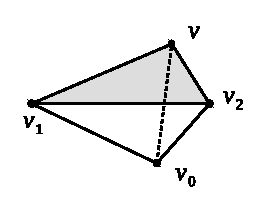
\includegraphics[width=.5\textwidth]{figures/tetrahedron.eps}
    \caption{Tetrahedral volume}
    \label{fig:tetrahedron}
\end{figure}

Given four vertices $(v, v_0, v_1, v_2)$ of a tetrahedron the volume can be calculated with the left hand side of \cref{eq:tetrahedron_volume}. If this volume is zero there is no local change in volume and therefore no global change in volume, hence, the right hand side is set to zero.

\begin{equation} \label{eq:tetrahedron_volume}
\norm*{\frac{(v - v_0) \cdot ((v_1-v_0) \times (v_2 - v_0))}{6}} = 0
\end{equation}

\cref{eq:tetrahedron_volume} can be rewritten as 

\begin{equation} \label{eq:tetrahedron_volume_rewritten}
\frac{area}{3} \mathbf{n}^\intercal \mathbf{v} - \frac{area}{3} \mathbf{n}^\intercal \mathbf{v}_0 = \mathbf{g}_{vol}^\intercal \mathbf{v} + d_{vol} = 0
\end{equation}


where $v_0$ is a vertex of face $(v_0, v_1, v_2)$, $n^\intercal$ is the face normal, and $v$ is the new vertex position. This will give a linear constraint that can easily be added to the system of linear equations, thus, increasing its dimension by one.

\begin{equation} \label{eq:volume_constraint}
  \begin{bmatrix}
    \mathbf{A}                & \mathbf{g}_{vol} \\
     \mathbf{g}_{vol}^\intercal & 0
  \end{bmatrix}
  \begin{bmatrix}
    \mathbf{v}_{min} \\
    \gamma
  \end{bmatrix}
  =
  \begin{bmatrix}
    -\mathbf{b} \\
    -d_{vol}
  \end{bmatrix}
\end{equation}


\subsection{Improving Texture Atlas}
Trying to keep the seam during simplification improves the quality of the resulting mesh. However, when a mesh is heavily simplified it is hard to keep the geometry and often gives a bad result. Removing the seam constraint gives a better geometry but now there is another problem. Since the seam is not kept we could get texture coordinates that lies outside the defined areas of the texture atlas. A common color in this area is black but it depends on what the texture artist chose.

One way of finding valid pixels is to first create a mesh where vertices are defined by the texture coordinates, i.e. $v = (s, t, 0)$ where $s$, and $t$ are the texture coordinates. This creates sheets lying in the same plane where empty areas will be locations that are not defined in the texture atlas. By casting rays towards the cheats the empty areas can be detected. The origin of the rays will be based on the pixel locations but translated in the direction of the normal to the plane. They will then be casted straight down towards the sheets and if they hit anything we have found a valid pixel.

Given some scattered data, Gortler et al. \cite{Gortler96thelumigraph} present a way of filling in the empty areas based on the given data. This is done by using a image pyramid containing images of decreasing resolution. The lower resolution images is used to fill in the empty areas of the higher resolution images. The algorithm works in the two phases \emph{pull} and \emph{push} hence it is given the name \emph{pull-push}.

\begin{subs}
\subsubsection{Pull}
The first level $r = 0$ of the pyramid is the input image and level $r + 1$ have half the size of level $r$ in each dimension. Each pixel have a data value $x^r_i$ and weight $w^r_i$. The pull phase starts at level 0 and recursively computes the values of the next level according to \cref{eq:pull_x,eq:pull_w} where $\tilde{h}$ is a gaussian filter. $\tilde{h}$ blends the neighboring pixels with an applied weight according to \cref{fig:pull_filter} which will give a blurred image. At the first level valid pixels is assigned a weight of $1$ and invalid pixels a weight of $0$. This will make sure that the valid pixels will not be changed.

\begin{align}
  w^{r+1}_i &= \sum_k {\tilde{h}_k \min(w^r_k,1)} \label{eq:pull_x}\\
  x^{r+1}_i &= \frac{1}{w^{r+1}_i} \sum_k {\tilde{h}_k \min(w^r_k,1) x^r_i} \label{eq:pull_w}
\end{align}



\begin{figure}[h]
    \centering
    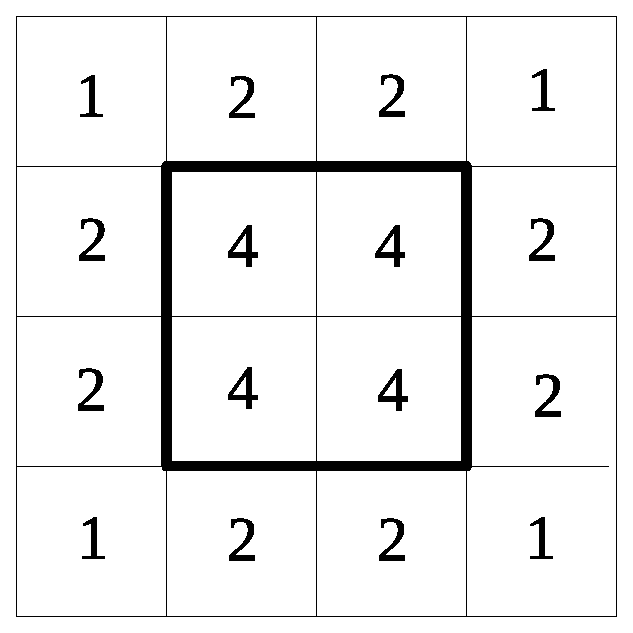
\includegraphics[width=.3\textwidth]{figures/pull_filter.eps}
    \caption{Interpolation of pixel values in pull phase}
    \label{fig:pull_filter}
\end{figure}
\end{subs}

\begin{subs}
\subsubsection{Push}
The lower resolution images generated in the pull phase are used in the push phase to fill in empty pixels in the higher resolution images. The weights that was computed for each pixel in the pull phase are used to determine how the pixel values will be blended. A lower weight means that the color will mostly be influenced by the lower resolution pixels. Higher weights means that the current pixel color will influence the most.

The first step is to calculate temporay values $tx$ and $tw$ according to
\begin{align}
  tw^{r}_i &= \sum_k {h_k \min(w^{r+1}_k,1)} \label{eq:push_tw}\\
  tx^{r}_i &= \frac{1}{tw^{r}_i} \sum_k {h_k \min(w^{r+1}_k,1) x^{r+1}_i} \label{eq:push_tx}
\end{align}

The current values $x^r$ and $w^r$ are then blended with the temporary values according to
\begin{align}
  x^r_i &= tx^r_i (1 - w^r_i) + w^r x^r_i \label{eq:push_x}\\
  w^r_i &= tw^r_i (1 - w^r_i) + w^r \label{eq:push_w}
\end{align}

What neighboring pixels to blend with is determined by the pixel's location within its superpixel. For example, the top-left subpixel of the middle pixel is blended with the top-left, top, middle, and left pixel as can be seen in \cref{fig:push_filter}. These pixel values are weighted by $1$, $3$, or $9$,  depending on their location.

\begin{figure}[h]
    \centering
    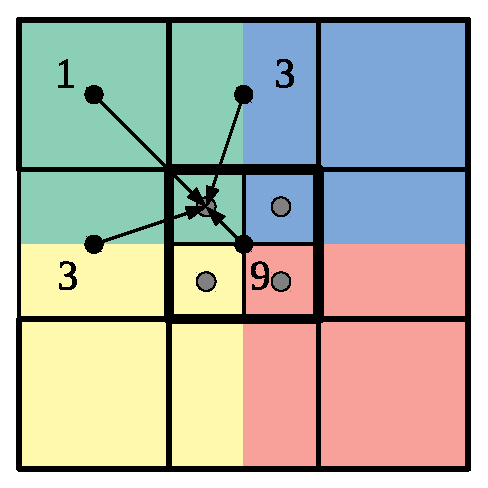
\includegraphics[width=.5\textwidth]{figures/push_filter_color.eps}
    \caption{Interpolation of pixel values in push phase}
    \label{fig:push_filter}
\end{figure}

\end{subs}

 Pixels at the edges of the texture needs special treatment since some neighboring pixels are missing. There exist multiple solutions to this problem such as ignoring pixels, using the value of the closest pixel, mirroring values, or wrapping around to the opposite side. Textures are often wrapped when used and therefore the wrapping seams like a good solution.

 
\clearpage

%\begin{equation}
  
%\end{equation}


%%%%%%%%%%%%%%%%%%%%%%%%%%%%%%%%%%%%%%%%%%%%%%%%%%%%%%%%%%%%%%%%%%%%%%
%%
%%% Evaluation
%%
%%%%%%%%%%%%%%%%%%%%%%%%%%%%%%%%%%%%%%%%%%%%%%%%%%%%%%%%%%%%%%%%%%%%%%
\section{Evaluation} \label{sec:evaluation}
An evaluation of the appearance of meshes simplified by the implemented simplification scheme was performed. In this section the the models and metrics used for the evaluation is presented.

\subsection{Models}
Four LoD:s are usually used by Configura and they are defined by triangle density ($\#triangles/area$). The four levels are super (5000 $triangles/m^2$), high (1000 $triangles/m^2$), medium (200 $triangles/m^2$), and low  (50 $triangles/m^2$) and these will be used for the evaluation. Configura have textured models of humans and a subset of them have been selected to be used in the evaluation. The triangle counts lies around 15000 but smaller models with about 10000 and larger models with about 30000 triangles are also included. 

\subsection{Appearance Preservation}
In order to compare how well the appearance is preserved for different LoDs the image metric described in \cref{sec:metrics_for_appearance_preservation} can be used. The main idea is to render multiple images of both the original and simplified mesh from a set of camera positions defined by the vertices of a rhombicuboctahedron (\cref{fig:rhombicuboctahedron}). A RMS of all the pixel values of the images is then simply the error that the simplification introduced. The authors \cite{lindstrom2000image} measured difference in luminance but other metrics, such as Euclidean distance of the RGB colors, can be used.



Another common approach for measuring the difference between two meshes is to use the \emph{Hausdorff distance}. Cignoni et al. \cite{cignoni1998metro} first defines the distance between a point $p$ and a surface $S$ as

\[e(p, S) = \min_{p' \in S} \norm*{p' - p}\]

A one-sided distance between two surfaces \(S, S'\) is then defined as

\[E(S, S') = \max_{p \in S} e(p, S')\]

This distance is not symmetric and depends on which surface you start the measurement from, meaning that \(E(S, S') \neq E(S', S)\) in some cases. Finally, the Hausdorff distance can be obtained by taking the maximum of the distances in both directions. A mean distance between the surfaces can be obtained by uniformly sample points on both surfaces, measuring their Hausdorff distance, and then dividing by the number of sampled points.

How many points to sample depends on the size and shape of the meshes being compared. For the meshes used in the evaluation 10000 points on each mesh seamed to give a stable estimate of the error introduced by the simplification.

The sampling of a point on a mesh can be done in two steps: First, randomly pick a triangle of the mesh, then pick a random point on the chosen triangle. A triangle can simply be picked by uniformly choose a random triangle index. A random point on a triangle can be picked by using barycentric coordinates. As can be seen in \cref{lst:sample_point}, two random numbers \(s, t\) between 0 and 1 are chosen. The sampled point is then a convex combination of the vertices \((v_0, v_1, v_2)\) of the triangle. The condition \(s + t \leq 1\) must be fulfilled, therefore, $s$ and $t$ are randomized until the condition is met.  

\begin{minipage}{\textwidth}
  \begin{lstlisting}[caption={Sampling point on triangle by using barycentric coordinates}, label={lst:sample_point}]
    do {
      float s = random(0,1);
      float t = random(0,1);
    } while (s + t > 1)

    point v = (1 - s - t)*v0 + s*v1 + t*v2;
  \end{lstlisting}
\end{minipage}

\subsection{Volume preservation} \label{sec:computing_volume}
Since the volume of a mesh is affected by simplification a way to measure the volume is needed. \emph{Zhang and Chen} \cite{zhang2001efficient} introduce a way of measuring the volume of a manifold mesh using tetrahedrons. A tetrahedron have 4 vertices, therefore, they can be created by using the vertices of a triangle and the origin. As explained in \cref{sec:volume_preservation} the volume of a tetrahedron can be calculated with \cref{eq:tetrahedron_volume}. Not taking the absolute value of the equation gives the \emph{signed volume} which is used by Zhang and Chen. As can be seen in \cref{fig:mesh_volume} triangles with a normal facing the origin gets a negative volume and triangles facing away from the origin get a positive volume. By taking the sum of all the tetrahedrons, constructed from the triangles and the origin, the volume contained within the triangles is obtained. As said before this only works if the mesh is manifold.

\begin{align}
  V_i &= \frac{v_0 \cdot (v_1 \times v_2)}{6}\\
  V_{total} &= \sum_i{V_i}
\end{align}

\begin{figure}[h]
  \centering
  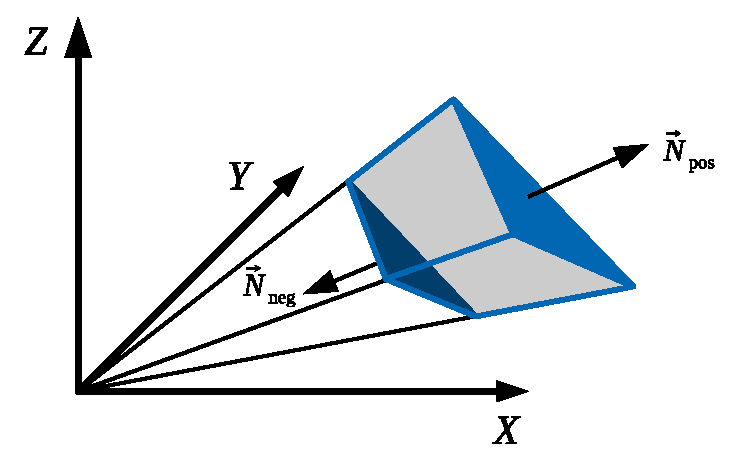
\includegraphics[width=\textwidth]{mesh_volume.eps}
  \caption{Illustration of mesh volume computation}
  \label{fig:mesh_volume}
  \end{figure}


\subsection{Execution Time} \label{sec:computation_time}
A simple parallelization with OpenMP have been implemented with the goal of decreasing the computation time. In order to see how much the computation time is reduced it was measured for multiple runs of the simplification scheme using the office woman model. Measurements was made for the four LoD:s super, high, medium, and low and the number used threads was from 1 to 8 threads.

To account for noise the measurements of the execution time is performed several times. From the collected data the mean \(\bar{x}\) and standard deviation \(s\) can be calculated. The confidence interval \([a, b]\) fo the execution time can be found by the equations shown in \cref{sec:measuring_algorithmic_performance} with \(\alpha = 0.05\).


\iffalse
An important property of a mesh simplification algorithm is the time it takes to simplify a full-resolution mesh to a lower-resolution mesh. While this doesn't impact the run-time of the mesh (that is accounted for by the rendering time, measured in Section~\ref{sec:rendering_time}), it is still important to reduce it as much as possible. This is especially true if the LoD is dynamically generated at run-time, but it is also important since many more meshes can be simplified per time unit (important if a simplifier is to be provided as a service, as \emph{Simplygon Linköping} does).

In order to compare the execution time of different number of threads, they all target the same appearance thresholds as specified in Section~\ref{sec:appearance_preservation} by tweaking the parameters unique to each algorithm. We then measure the time it takes for the simplification algorithm to execute when using these parameters, in other words, simply by: \(time_\mathcal{A} = end_\mathcal{A} - start_\mathcal{A}\) for an algorithm \(\mathcal{A}\). Of course, this measurement is done several times to account for noise. After calculating the mean \(\bar{x}\) and the standard-deviation \(s\), one can find the confidence interval \([a, b]\) of the execution time by the equations shown in Section~\ref{sec:measuring_algorithmic_performance} with 19 degrees of freedom and \(\alpha = 5 \%\).
\fi

%\subsection{Computation Time}
%\subsection{Memory Usage}
%\subsection{Rendering Time}


\iffalse
In order to determine which of these algorithms provide the best performance for a target appearance threshold, an evaluation of the polygon count, computation time, memory usage and rendering time of the simplified mesh is done for each of the implemented solutions. In the results from this step, a series of tables are generated to compare the performance between the algorithms by using a common comparison framework. In this section, we describe this common comparison framework and then show how we can measure each of the parameters.

In essence, this is done by targeting a certain appearance threshold, tweaking the mesh simplification algorithm's parameters to achieve this threshold, and then measuring the given performance. This gives a universal measure of ``quality'' for all of the algorithms, which would otherwise have different error metrics used for applying the simplification. Since the performance measures are noisy, a total of \(n=20\) samples will be taken. According to \emph{David Lilja}~\cite[p.~50]{lilja2005measuring} the t-student distribution should be used when \(n < 30\), as shown in Section~\ref{sec:measuring_algorithmic_performance}.

The pack of test meshes that are going to be used in the comparison are a combination of textured models provided by Configura and others taken from the public domain. The exact selection of these is still to be decided, but should include both low- \& high-polygon meshes.
\fi

\iffalse
\subsection{Appearance Preservation} \label{sec:appearance_preservation}
In order to compare the appearance preservation of the mesh simplification algorithms, the image-metric explained in section~\ref{sec:metrics_for_appearance_preservation} is used. It is useful since it can compare the difference of any two meshes, therefore, it does not depend on the algorithm used.

For both the original mesh and a simplified mesh, 24 images with resolution $512 \times 512$ is rendered with a simple renderer based on \emph{OpenGL}. The camera is placed at the vertices of a rhombicuboctahedron and is faced towards the center where the mesh is placed. A light source is placed at the camera position. This will make sure that the surface facing the camera will be illuminated.

The two sets of 24 images each is used to compute the RMS of the simplified mesh with equation~\ref{eq:rms_image_sets}. This RMS value can then be used to compare how well the algorithms perform. 
\subsection{Polygon Count} \label{sec:polygon_count}
Concerning research question 3, the appearance preservation for a specific target polygon count needs to be measured. Therefore, the simplification algorithms is tasked to simplify until the target polygon count is reached. When it is reached, the image-metric is used to measure how well the appearance is preserved. Measurements will be performed for multiple target polygon counts. 

\subsection{Computation Time} \label{sec:computation_time}

An important property of a mesh simplification algorithm is the time it takes to simplify a full-resolution mesh to a lower-resolution mesh. While this doesn't impact the run-time of the mesh (that is accounted for by the rendering time, measured in Section~\ref{sec:rendering_time}), it is still important to reduce it as much as possible. This is especially true if the LoD is dynamically generated at run-time, but it is also important since many more meshes can be simplified per time unit (important if a simplifier is to be provided as a service, as \emph{Simplygon Linköping} does).

In order to compare the execution time of the different algorithms, they all target the same appearance thresholds as specified in Section~\ref{sec:appearance_preservation} by tweaking the parameters unique to each algorithm. We then measure the time it takes for the simplification algorithm to execute when using these parameters, in other words, simply by: \(time_\mathcal{A} = end_\mathcal{A} - start_\mathcal{A}\) for an algorithm \(\mathcal{A}\). Of course, this measurement is done several times to account for noise. After calculating the mean \(\bar{x}\) and the standard-deviation \(s\), one can find the confidence interval \([a, b]\) of the execution time by the equations shown in Section~\ref{sec:measuring_algorithmic_performance} with 19 degrees of freedom and \(\alpha = 5 \%\).

\subsection{Memory Usage} \label{sec:memory_usage}

Another important performance property of the algorithm is the accumulated memory used when simplifying the mesh. Depending on the size of the mesh in triangles, the algorithm could consume large amounts of memory (and might not even fit in the primary memory in some cases). It is therefore important to compare the simplification algorithms to determine those which are suited for optimizing large triangle meshes and those that aren't. Since this measure will always be deterministic (at least for the method we use to measure it), there is no need to apply any statistical measures. The \emph{Valgrind} suite was chosen since it has the \emph{Massif} heap profiler, which gives accurate memory usage. According to the \emph{Massif documentation}~\cite{valgrind2017manual} there is an expected slowdown of 20x, which isn't a problem since the computation time and rendering time are measured separately. Below are the commands to find the memory usage.

\begin{lstlisting}[language=bash]
  (*\textbf{valgrind}*) --tool=massif (*\textit{./simplify --algorithm=<algorithm> <input-mesh> <output-mesh>}*)
\end{lstlisting}

\subsection{Rendering Time} \label{sec:rendering_time}
One main purpose of simplifying a mesh is to reduce the rendering time. Therefore, the frame rate is measured when rendering the original mesh and the simplified meshes. The simplified meshes comes from the previous steps where different appearance-thresholds was targeted. Frame rate is measured by counting how many frames that have been rendered during a period of one second. As with computation time, this measurement may have noise and therefore multiple samples needs to be obtained. The mean and confidence interval is obtained in the same way.
\fi

%%%%%%%%%%%%%%%%%%%%%%%%%%%%%%%%%%%%%%%%%%%%%%%%%%%%%%%%%%%%%%%%%%%%%%
%%% method.tex ends here

%%% Local Variables: 
%%% mode: latex
%%% TeX-master: "thesis"
%%% End: 
